% \vspace{-1em}
\section{Introducción}
\label{sec:intro}

El campo de los large multimodal models (LMMs) ha experimentado un progreso enorme en los últimos años. El trabajo seminal de LLaVA \cite{liu2024visual} transfirió con éxito el poder de la predicción autoregresiva del siguiente token desde los large language models (LLMs) \cite{OpenAI_ChatGPT_Website, achiam2023gpt, touvron2023llama, bai2023qwen, jiang2023mistral} al dominio multimodal, estableciendo un nuevo estándar para la comprensión visual al modelar de forma autoregresiva tokens visuales y de lenguaje mediante capas de causal transformer. Desde entonces, los LMMs basados en Transformer han sido ampliamente estudiados y mejorados para abordar una gama diversa de tareas, como comprensión de imágenes de alta resolución \cite{llavanext2024, laurenccon2024matters, wang2024qwen2} y razonamiento intercalado image-text \cite{jiang2024mantis, li2024llava, li2024llavaov}. Sin embargo, la complejidad cuadrática inherente a las operaciones de causal self-attention presenta desafíos significativos para entradas de contexto largo, lo que dificulta que los LMMs basados en Transformer manejen eficazmente la tarea de comprender videos extremadamente largos.

\begin{figure}[t!]
    \centering
    
    \begin{subfigure}[b]{0.9\linewidth}
        \centering
        \vspace{-2pt}
        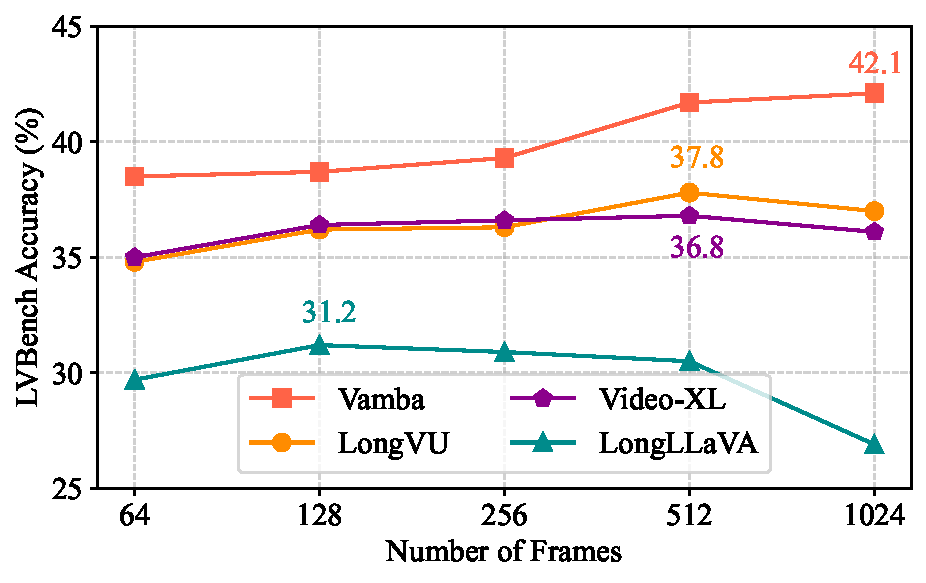
\includegraphics[width=\linewidth]{figures/lvbench.pdf}
        \label{fig:lvbench}
    \end{subfigure}
    
    \vspace{-1.5em}
    
    \begin{subfigure}[b]{1\linewidth}
        \centering
        \vspace{-2pt}
        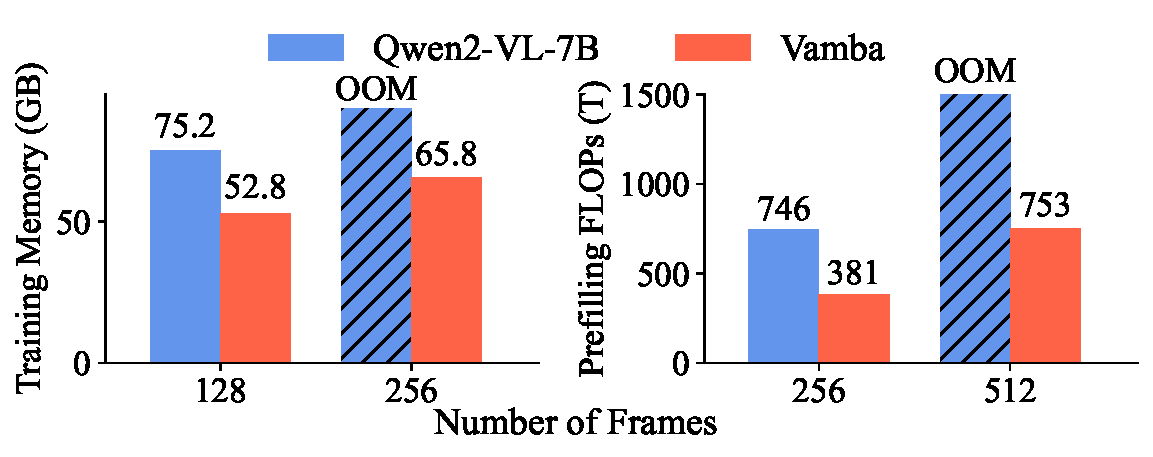
\includegraphics[width=\linewidth]{figures/compare.pdf}
        \label{fig:compare}
    \end{subfigure}
    \vspace{-3.5em}
    \caption{\model logra un sólido rendimiento en comprensión de video largo (42.1\% en LVBench \cite{wang2024lvbench}) mientras es más eficiente computacionalmente en comparación con los LMMs basados en Transformer.}
    \label{fig:teaser}
    \vspace{-1.5em}
\end{figure}

Un desafío clave para los LMMs avanzados al procesar entradas de video largas es que tienden a codificar cada frame en una gran cantidad de vision tokens, lo que genera costos sustanciales de cómputo y memoria tanto durante el entrenamiento como en la inferencia. Por ejemplo, Qwen2-VL~\citep{wang2024qwen2} solo puede procesar 256 frames (360p) en una sola GPU, lo cual está lejos de ser suficiente para la comprensión de videos de una hora. Para reducir el costo computacional/de memoria, los esfuerzos previos se han centrado principalmente en reducir los vision tokens en la secuencia de entrada. Varios enfoques \cite{zhang-etal-2023-video, li2023videochat, li2024mvbench, fei2024video} utilizan un Q-Former \cite{li2023blip} para comprimir vision tokens. Métodos más recientes, como LongVU \cite{shen2024longvu} y Video-XL \cite{shu2024video}, particionan las secuencias de vision tokens en chunks y emplean mecanismos adaptativos de compresión de tokens para disminuir el conteo. Otra línea de trabajo, como InternVideo2.5~\citep{internvideo2_5} y Orxy-1.5~\citep{liu2024oryx}, emplea diversos mecanismos para evaluar la importancia de los vision tokens y así descartar o fusionar aquellos menos significativos \cite{tokenmerging} durante el entrenamiento y la inferencia. A pesar de estos avances, siguen existiendo desafíos clave en los LMMs para comprensión de video largo. Primero, una reducción agresiva de tokens puede provocar pérdida crítica de información, particularmente al procesar videos extremadamente largos. Segundo, estos métodos siguen sufriendo complejidad computacional cuadrática a medida que aumenta el número de frames de entrada. Tercero, los métodos basados en reducción de tokens requieren sobrecarga adicional, lo que puede incrementar el wall-clock time real.

\begin{table}[]
\centering
\small
\caption{Complejidad teórica de tiempo y memoria para LMMs basados en Transformer y \model en pre-filling. $M$ y $N$ representan el número de vision y text tokens. $d$ denota la dimensión oculta.}
% , C is a small constant. In hour-long video benchmarks, we have $M \gg N \approx d$, $M$ could be at least 100x larger than $N$. }
\setlength\tabcolsep{7 pt}
\begin{tabular}{l|c|c}
\toprule
Model                  & Time Complexity & Memory Complexity \\ \midrule
Transformer            &     $O(d(M+N)^2)$             &   $O((M+N)^2)$             \\
\model                 &   $O(dMN+d^2 M)$              &   $O(MN)$                \\
% \midrule
% $\text{Ratio} = \frac{\text{\model}}{\text{Transformer}}$  &   $O(\frac{N + d}{M + 2N + C})$   &   $O(\frac{N}{M + 2N + C})$  \\
\bottomrule
\end{tabular}
\label{tab:complexity}
\vspace{-1.5em}
\end{table}


En este estudio investigamos una dirección ortogonal a los enfoques previos: en lugar de comprimir los video tokens, buscamos desarrollar una arquitectura de modelo alternativa que mejore la eficiencia del procesamiento de video tokens durante el entrenamiento y la etapa de pre-filling de la inferencia. Proponemos \model, un modelo híbrido Mamba-Transformer para comprensión eficiente de videos de una hora. La idea clave de nuestro método es que podemos diseñar módulos eficientes para aproximar la operación de causal self-attention tanto para tokens de texto como de video en LMMs basados en Transformer. En particular, proponemos (1) utilizar cross-attentions para actualizar los tokens de texto a partir de video tokens, lo cual es asequible debido a la corta longitud de los tokens de texto, y (2) adoptar Mamba-2~\citep{dao2024transformers} para procesar la enorme cantidad de video tokens con complejidad lineal.

Suponiendo una secuencia de entrada combinada de $M+N$ tokens, donde $M$ es el número de video tokens y $N$ el número de tokens de texto, encontramos que $M$ puede ser al menos 100 veces mayor que $N$ en muchas tareas de video largo ($M \gg N$). Nuestro modelo puede reducir la complejidad computacional de entrenamiento/pre-filling de $O(d(M+N)^2)$ a $O(dMN+d^2M)$, donde $d$ es la dimensión oculta, según la Tabla~\ref{tab:complexity}. En la práctica, esta mejora teórica puede no materializarse por completo debido a la suboptimización de hardware para Mamba~\citep{gu2023mamba}. Aun así, observamos una reducción de más del 50\% en uso de memoria GPU y FLOPs/runtime durante entrenamiento e inferencia para entradas de video largas, como se muestra en la Figura~\ref{fig:teaser}. \model puede entrenarse eficientemente usando 8$\times$A800 GPUs, mientras que otros video LMMs eficientes como LongVU \cite{shen2024longvu} y LongLLaVA \cite{wang2024longllava} requieren 64 y 24 GPUs para el entrenamiento, respectivamente. Mediante un entrenamiento en dos etapas, nuestro \model logra una mejora del 4.3\% sobre los mejores video LMMs eficientes en el desafiante benchmark de comprensión de video de una hora LVBench \cite{wang2024lvbench}. En otros datasets de comprensión de video largo como Video-MME~\citep{fu2024video}, MLVU~\citep{zhou2024mlvu} y LongVideoBench~\citep{wu2025longvideobench}, \model también alcanza un rendimiento sobresaliente.

\noindent Nuestras contribuciones pueden resumirse como sigue:
\begin{itemize}
    \item [1.] Proponemos \model, un modelo híbrido Mamba-Transformer para comprensión de videos de una hora. El diseño de \model incorpora módulos eficientes como bloques Mamba-2 y capas cross-attention, reduciendo efectivamente la sobrecarga computacional de los LMMs basados en Transformer.
    \item [2.] Realizamos un estudio de ablación exhaustivo y mostramos que emplear bloques Mamba-2 e inicializar los pesos de cross-attention a partir de capas self-attention preentrenadas es crucial para lograr alto rendimiento en \model.
    \item [3.] Nuestras evaluaciones extensivas demuestran que \model logra sólidas capacidades de comprensión de video. En particular, \model obtiene una mejora del 4.3\% sobre los video LMMs eficientes de estado del arte en el desafiante benchmark de una hora LVBench.
\end{itemize}
